% Created by tikzDevice version 0.12.3 on 2020-02-05 13:45:15
% !TEX encoding = UTF-8 Unicode
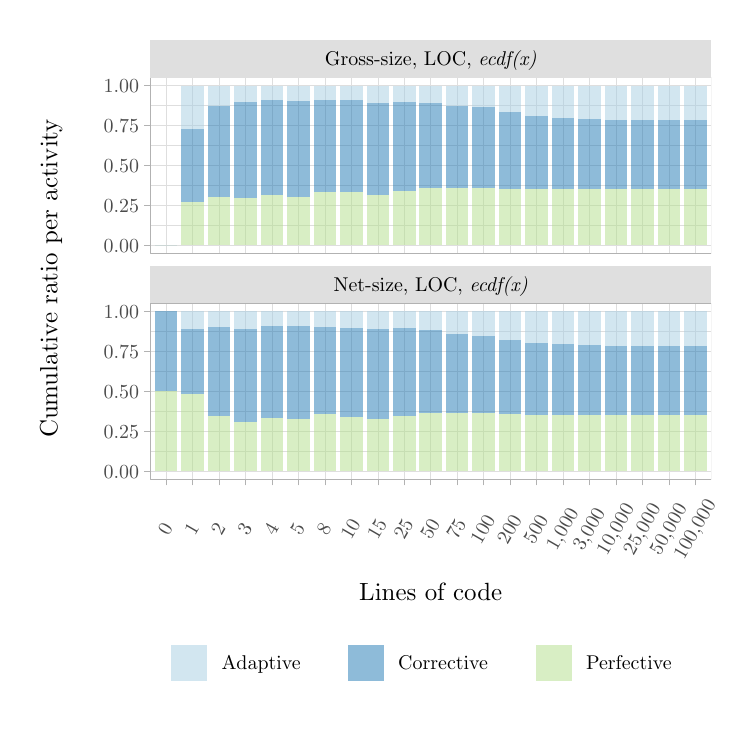
\begin{tikzpicture}[x=1pt,y=1pt]
\definecolor{fillColor}{RGB}{255,255,255}
\path[use as bounding box,fill=fillColor,fill opacity=0.00] (0,0) rectangle (251.50,245.72);
\begin{scope}
\path[clip] (  0.00,  0.00) rectangle (251.50,245.72);
\definecolor{drawColor}{RGB}{255,255,255}
\definecolor{fillColor}{RGB}{255,255,255}

\path[draw=drawColor,line width= 0.5pt,line join=round,line cap=round,fill=fillColor] (  0.00,  0.00) rectangle (251.50,245.72);
\end{scope}
\begin{scope}
\path[clip] ( 44.29,164.14) rectangle (247.00,227.66);
\definecolor{fillColor}{RGB}{255,255,255}

\path[fill=fillColor] ( 44.29,164.14) rectangle (247.00,227.66);
\definecolor{drawColor}{gray}{0.87}

\path[draw=drawColor,line width= 0.1pt,line join=round] ( 44.29,174.25) --
	(247.00,174.25);

\path[draw=drawColor,line width= 0.1pt,line join=round] ( 44.29,188.68) --
	(247.00,188.68);

\path[draw=drawColor,line width= 0.1pt,line join=round] ( 44.29,203.12) --
	(247.00,203.12);

\path[draw=drawColor,line width= 0.1pt,line join=round] ( 44.29,217.55) --
	(247.00,217.55);

\path[draw=drawColor,line width= 0.2pt,line join=round] ( 44.29,167.03) --
	(247.00,167.03);

\path[draw=drawColor,line width= 0.2pt,line join=round] ( 44.29,181.46) --
	(247.00,181.46);

\path[draw=drawColor,line width= 0.2pt,line join=round] ( 44.29,195.90) --
	(247.00,195.90);

\path[draw=drawColor,line width= 0.2pt,line join=round] ( 44.29,210.34) --
	(247.00,210.34);

\path[draw=drawColor,line width= 0.2pt,line join=round] ( 44.29,224.77) --
	(247.00,224.77);

\path[draw=drawColor,line width= 0.2pt,line join=round] ( 50.03,164.14) --
	( 50.03,227.66);

\path[draw=drawColor,line width= 0.2pt,line join=round] ( 59.59,164.14) --
	( 59.59,227.66);

\path[draw=drawColor,line width= 0.2pt,line join=round] ( 69.15,164.14) --
	( 69.15,227.66);

\path[draw=drawColor,line width= 0.2pt,line join=round] ( 78.72,164.14) --
	( 78.72,227.66);

\path[draw=drawColor,line width= 0.2pt,line join=round] ( 88.28,164.14) --
	( 88.28,227.66);

\path[draw=drawColor,line width= 0.2pt,line join=round] ( 97.84,164.14) --
	( 97.84,227.66);

\path[draw=drawColor,line width= 0.2pt,line join=round] (107.40,164.14) --
	(107.40,227.66);

\path[draw=drawColor,line width= 0.2pt,line join=round] (116.96,164.14) --
	(116.96,227.66);

\path[draw=drawColor,line width= 0.2pt,line join=round] (126.52,164.14) --
	(126.52,227.66);

\path[draw=drawColor,line width= 0.2pt,line join=round] (136.09,164.14) --
	(136.09,227.66);

\path[draw=drawColor,line width= 0.2pt,line join=round] (145.65,164.14) --
	(145.65,227.66);

\path[draw=drawColor,line width= 0.2pt,line join=round] (155.21,164.14) --
	(155.21,227.66);

\path[draw=drawColor,line width= 0.2pt,line join=round] (164.77,164.14) --
	(164.77,227.66);

\path[draw=drawColor,line width= 0.2pt,line join=round] (174.33,164.14) --
	(174.33,227.66);

\path[draw=drawColor,line width= 0.2pt,line join=round] (183.89,164.14) --
	(183.89,227.66);

\path[draw=drawColor,line width= 0.2pt,line join=round] (193.45,164.14) --
	(193.45,227.66);

\path[draw=drawColor,line width= 0.2pt,line join=round] (203.02,164.14) --
	(203.02,227.66);

\path[draw=drawColor,line width= 0.2pt,line join=round] (212.58,164.14) --
	(212.58,227.66);

\path[draw=drawColor,line width= 0.2pt,line join=round] (222.14,164.14) --
	(222.14,227.66);

\path[draw=drawColor,line width= 0.2pt,line join=round] (231.70,164.14) --
	(231.70,227.66);

\path[draw=drawColor,line width= 0.2pt,line join=round] (241.26,164.14) --
	(241.26,227.66);
\definecolor{fillColor}{RGB}{178,223,138}

\path[fill=fillColor,fill opacity=0.50] ( 45.97,167.03) rectangle ( 54.10,167.03);
\definecolor{fillColor}{RGB}{31,120,180}

\path[fill=fillColor,fill opacity=0.50] ( 45.97,167.03) rectangle ( 54.10,167.03);
\definecolor{fillColor}{RGB}{166,206,227}

\path[fill=fillColor,fill opacity=0.50] ( 45.97,167.03) rectangle ( 54.10,167.03);
\definecolor{fillColor}{RGB}{178,223,138}

\path[fill=fillColor,fill opacity=0.50] ( 55.53,167.03) rectangle ( 63.66,182.78);
\definecolor{fillColor}{RGB}{31,120,180}

\path[fill=fillColor,fill opacity=0.50] ( 55.53,182.78) rectangle ( 63.66,209.02);
\definecolor{fillColor}{RGB}{166,206,227}

\path[fill=fillColor,fill opacity=0.50] ( 55.53,209.02) rectangle ( 63.66,224.77);
\definecolor{fillColor}{RGB}{178,223,138}

\path[fill=fillColor,fill opacity=0.50] ( 65.09,167.03) rectangle ( 73.22,184.60);
\definecolor{fillColor}{RGB}{31,120,180}

\path[fill=fillColor,fill opacity=0.50] ( 65.09,184.60) rectangle ( 73.22,217.24);
\definecolor{fillColor}{RGB}{166,206,227}

\path[fill=fillColor,fill opacity=0.50] ( 65.09,217.24) rectangle ( 73.22,224.77);
\definecolor{fillColor}{RGB}{178,223,138}

\path[fill=fillColor,fill opacity=0.50] ( 74.65,167.03) rectangle ( 82.78,184.09);
\definecolor{fillColor}{RGB}{31,120,180}

\path[fill=fillColor,fill opacity=0.50] ( 74.65,184.09) rectangle ( 82.78,218.87);
\definecolor{fillColor}{RGB}{166,206,227}

\path[fill=fillColor,fill opacity=0.50] ( 74.65,218.87) rectangle ( 82.78,224.77);
\definecolor{fillColor}{RGB}{178,223,138}

\path[fill=fillColor,fill opacity=0.50] ( 84.21,167.03) rectangle ( 92.34,185.24);
\definecolor{fillColor}{RGB}{31,120,180}

\path[fill=fillColor,fill opacity=0.50] ( 84.21,185.24) rectangle ( 92.34,219.44);
\definecolor{fillColor}{RGB}{166,206,227}

\path[fill=fillColor,fill opacity=0.50] ( 84.21,219.44) rectangle ( 92.34,224.77);
\definecolor{fillColor}{RGB}{178,223,138}

\path[fill=fillColor,fill opacity=0.50] ( 93.78,167.03) rectangle (101.90,184.50);
\definecolor{fillColor}{RGB}{31,120,180}

\path[fill=fillColor,fill opacity=0.50] ( 93.78,184.50) rectangle (101.90,219.07);
\definecolor{fillColor}{RGB}{166,206,227}

\path[fill=fillColor,fill opacity=0.50] ( 93.78,219.07) rectangle (101.90,224.77);
\definecolor{fillColor}{RGB}{178,223,138}

\path[fill=fillColor,fill opacity=0.50] (103.34,167.03) rectangle (111.46,186.19);
\definecolor{fillColor}{RGB}{31,120,180}

\path[fill=fillColor,fill opacity=0.50] (103.34,186.19) rectangle (111.46,219.52);
\definecolor{fillColor}{RGB}{166,206,227}

\path[fill=fillColor,fill opacity=0.50] (103.34,219.52) rectangle (111.46,224.77);
\definecolor{fillColor}{RGB}{178,223,138}

\path[fill=fillColor,fill opacity=0.50] (112.90,167.03) rectangle (121.03,186.28);
\definecolor{fillColor}{RGB}{31,120,180}

\path[fill=fillColor,fill opacity=0.50] (112.90,186.28) rectangle (121.03,219.46);
\definecolor{fillColor}{RGB}{166,206,227}

\path[fill=fillColor,fill opacity=0.50] (112.90,219.46) rectangle (121.03,224.77);
\definecolor{fillColor}{RGB}{178,223,138}

\path[fill=fillColor,fill opacity=0.50] (122.46,167.03) rectangle (130.59,185.15);
\definecolor{fillColor}{RGB}{31,120,180}

\path[fill=fillColor,fill opacity=0.50] (122.46,185.15) rectangle (130.59,218.51);
\definecolor{fillColor}{RGB}{166,206,227}

\path[fill=fillColor,fill opacity=0.50] (122.46,218.51) rectangle (130.59,224.77);
\definecolor{fillColor}{RGB}{178,223,138}

\path[fill=fillColor,fill opacity=0.50] (132.02,167.03) rectangle (140.15,186.76);
\definecolor{fillColor}{RGB}{31,120,180}

\path[fill=fillColor,fill opacity=0.50] (132.02,186.76) rectangle (140.15,219.02);
\definecolor{fillColor}{RGB}{166,206,227}

\path[fill=fillColor,fill opacity=0.50] (132.02,219.02) rectangle (140.15,224.77);
\definecolor{fillColor}{RGB}{178,223,138}

\path[fill=fillColor,fill opacity=0.50] (141.58,167.03) rectangle (149.71,187.68);
\definecolor{fillColor}{RGB}{31,120,180}

\path[fill=fillColor,fill opacity=0.50] (141.58,187.68) rectangle (149.71,218.65);
\definecolor{fillColor}{RGB}{166,206,227}

\path[fill=fillColor,fill opacity=0.50] (141.58,218.65) rectangle (149.71,224.77);
\definecolor{fillColor}{RGB}{178,223,138}

\path[fill=fillColor,fill opacity=0.50] (151.15,167.03) rectangle (159.27,187.74);
\definecolor{fillColor}{RGB}{31,120,180}

\path[fill=fillColor,fill opacity=0.50] (151.15,187.74) rectangle (159.27,217.54);
\definecolor{fillColor}{RGB}{166,206,227}

\path[fill=fillColor,fill opacity=0.50] (151.15,217.54) rectangle (159.27,224.77);
\definecolor{fillColor}{RGB}{178,223,138}

\path[fill=fillColor,fill opacity=0.50] (160.71,167.03) rectangle (168.83,187.84);
\definecolor{fillColor}{RGB}{31,120,180}

\path[fill=fillColor,fill opacity=0.50] (160.71,187.84) rectangle (168.83,217.04);
\definecolor{fillColor}{RGB}{166,206,227}

\path[fill=fillColor,fill opacity=0.50] (160.71,217.04) rectangle (168.83,224.77);
\definecolor{fillColor}{RGB}{178,223,138}

\path[fill=fillColor,fill opacity=0.50] (170.27,167.03) rectangle (178.40,187.47);
\definecolor{fillColor}{RGB}{31,120,180}

\path[fill=fillColor,fill opacity=0.50] (170.27,187.47) rectangle (178.40,215.12);
\definecolor{fillColor}{RGB}{166,206,227}

\path[fill=fillColor,fill opacity=0.50] (170.27,215.12) rectangle (178.40,224.77);
\definecolor{fillColor}{RGB}{178,223,138}

\path[fill=fillColor,fill opacity=0.50] (179.83,167.03) rectangle (187.96,187.51);
\definecolor{fillColor}{RGB}{31,120,180}

\path[fill=fillColor,fill opacity=0.50] (179.83,187.51) rectangle (187.96,213.85);
\definecolor{fillColor}{RGB}{166,206,227}

\path[fill=fillColor,fill opacity=0.50] (179.83,213.85) rectangle (187.96,224.77);
\definecolor{fillColor}{RGB}{178,223,138}

\path[fill=fillColor,fill opacity=0.50] (189.39,167.03) rectangle (197.52,187.37);
\definecolor{fillColor}{RGB}{31,120,180}

\path[fill=fillColor,fill opacity=0.50] (189.39,187.37) rectangle (197.52,213.06);
\definecolor{fillColor}{RGB}{166,206,227}

\path[fill=fillColor,fill opacity=0.50] (189.39,213.06) rectangle (197.52,224.77);
\definecolor{fillColor}{RGB}{178,223,138}

\path[fill=fillColor,fill opacity=0.50] (198.95,167.03) rectangle (207.08,187.29);
\definecolor{fillColor}{RGB}{31,120,180}

\path[fill=fillColor,fill opacity=0.50] (198.95,187.29) rectangle (207.08,212.58);
\definecolor{fillColor}{RGB}{166,206,227}

\path[fill=fillColor,fill opacity=0.50] (198.95,212.58) rectangle (207.08,224.77);
\definecolor{fillColor}{RGB}{178,223,138}

\path[fill=fillColor,fill opacity=0.50] (208.51,167.03) rectangle (216.64,187.27);
\definecolor{fillColor}{RGB}{31,120,180}

\path[fill=fillColor,fill opacity=0.50] (208.51,187.27) rectangle (216.64,212.39);
\definecolor{fillColor}{RGB}{166,206,227}

\path[fill=fillColor,fill opacity=0.50] (208.51,212.39) rectangle (216.64,224.77);
\definecolor{fillColor}{RGB}{178,223,138}

\path[fill=fillColor,fill opacity=0.50] (218.08,167.03) rectangle (226.20,187.28);
\definecolor{fillColor}{RGB}{31,120,180}

\path[fill=fillColor,fill opacity=0.50] (218.08,187.28) rectangle (226.20,212.41);
\definecolor{fillColor}{RGB}{166,206,227}

\path[fill=fillColor,fill opacity=0.50] (218.08,212.41) rectangle (226.20,224.77);
\definecolor{fillColor}{RGB}{178,223,138}

\path[fill=fillColor,fill opacity=0.50] (227.64,167.03) rectangle (235.76,187.28);
\definecolor{fillColor}{RGB}{31,120,180}

\path[fill=fillColor,fill opacity=0.50] (227.64,187.28) rectangle (235.76,212.41);
\definecolor{fillColor}{RGB}{166,206,227}

\path[fill=fillColor,fill opacity=0.50] (227.64,212.41) rectangle (235.76,224.77);
\definecolor{fillColor}{RGB}{178,223,138}

\path[fill=fillColor,fill opacity=0.50] (237.20,167.03) rectangle (245.33,187.28);
\definecolor{fillColor}{RGB}{31,120,180}

\path[fill=fillColor,fill opacity=0.50] (237.20,187.28) rectangle (245.33,212.41);
\definecolor{fillColor}{RGB}{166,206,227}

\path[fill=fillColor,fill opacity=0.50] (237.20,212.41) rectangle (245.33,224.77);
\definecolor{drawColor}{gray}{0.70}

\path[draw=drawColor,line width= 0.5pt,line join=round,line cap=round] ( 44.29,164.14) rectangle (247.00,227.66);
\end{scope}
\begin{scope}
\path[clip] ( 44.29, 82.56) rectangle (247.00,146.08);
\definecolor{fillColor}{RGB}{255,255,255}

\path[fill=fillColor] ( 44.29, 82.56) rectangle (247.00,146.08);
\definecolor{drawColor}{gray}{0.87}

\path[draw=drawColor,line width= 0.1pt,line join=round] ( 44.29, 92.67) --
	(247.00, 92.67);

\path[draw=drawColor,line width= 0.1pt,line join=round] ( 44.29,107.11) --
	(247.00,107.11);

\path[draw=drawColor,line width= 0.1pt,line join=round] ( 44.29,121.54) --
	(247.00,121.54);

\path[draw=drawColor,line width= 0.1pt,line join=round] ( 44.29,135.98) --
	(247.00,135.98);

\path[draw=drawColor,line width= 0.2pt,line join=round] ( 44.29, 85.45) --
	(247.00, 85.45);

\path[draw=drawColor,line width= 0.2pt,line join=round] ( 44.29, 99.89) --
	(247.00, 99.89);

\path[draw=drawColor,line width= 0.2pt,line join=round] ( 44.29,114.32) --
	(247.00,114.32);

\path[draw=drawColor,line width= 0.2pt,line join=round] ( 44.29,128.76) --
	(247.00,128.76);

\path[draw=drawColor,line width= 0.2pt,line join=round] ( 44.29,143.20) --
	(247.00,143.20);

\path[draw=drawColor,line width= 0.2pt,line join=round] ( 50.03, 82.56) --
	( 50.03,146.08);

\path[draw=drawColor,line width= 0.2pt,line join=round] ( 59.59, 82.56) --
	( 59.59,146.08);

\path[draw=drawColor,line width= 0.2pt,line join=round] ( 69.15, 82.56) --
	( 69.15,146.08);

\path[draw=drawColor,line width= 0.2pt,line join=round] ( 78.72, 82.56) --
	( 78.72,146.08);

\path[draw=drawColor,line width= 0.2pt,line join=round] ( 88.28, 82.56) --
	( 88.28,146.08);

\path[draw=drawColor,line width= 0.2pt,line join=round] ( 97.84, 82.56) --
	( 97.84,146.08);

\path[draw=drawColor,line width= 0.2pt,line join=round] (107.40, 82.56) --
	(107.40,146.08);

\path[draw=drawColor,line width= 0.2pt,line join=round] (116.96, 82.56) --
	(116.96,146.08);

\path[draw=drawColor,line width= 0.2pt,line join=round] (126.52, 82.56) --
	(126.52,146.08);

\path[draw=drawColor,line width= 0.2pt,line join=round] (136.09, 82.56) --
	(136.09,146.08);

\path[draw=drawColor,line width= 0.2pt,line join=round] (145.65, 82.56) --
	(145.65,146.08);

\path[draw=drawColor,line width= 0.2pt,line join=round] (155.21, 82.56) --
	(155.21,146.08);

\path[draw=drawColor,line width= 0.2pt,line join=round] (164.77, 82.56) --
	(164.77,146.08);

\path[draw=drawColor,line width= 0.2pt,line join=round] (174.33, 82.56) --
	(174.33,146.08);

\path[draw=drawColor,line width= 0.2pt,line join=round] (183.89, 82.56) --
	(183.89,146.08);

\path[draw=drawColor,line width= 0.2pt,line join=round] (193.45, 82.56) --
	(193.45,146.08);

\path[draw=drawColor,line width= 0.2pt,line join=round] (203.02, 82.56) --
	(203.02,146.08);

\path[draw=drawColor,line width= 0.2pt,line join=round] (212.58, 82.56) --
	(212.58,146.08);

\path[draw=drawColor,line width= 0.2pt,line join=round] (222.14, 82.56) --
	(222.14,146.08);

\path[draw=drawColor,line width= 0.2pt,line join=round] (231.70, 82.56) --
	(231.70,146.08);

\path[draw=drawColor,line width= 0.2pt,line join=round] (241.26, 82.56) --
	(241.26,146.08);
\definecolor{fillColor}{RGB}{178,223,138}

\path[fill=fillColor,fill opacity=0.50] ( 45.97, 85.45) rectangle ( 54.10,114.32);
\definecolor{fillColor}{RGB}{31,120,180}

\path[fill=fillColor,fill opacity=0.50] ( 45.97,114.32) rectangle ( 54.10,143.20);
\definecolor{fillColor}{RGB}{166,206,227}

\path[fill=fillColor,fill opacity=0.50] ( 45.97,143.20) rectangle ( 54.10,143.20);
\definecolor{fillColor}{RGB}{178,223,138}

\path[fill=fillColor,fill opacity=0.50] ( 55.53, 85.45) rectangle ( 63.66,113.25);
\definecolor{fillColor}{RGB}{31,120,180}

\path[fill=fillColor,fill opacity=0.50] ( 55.53,113.25) rectangle ( 63.66,136.78);
\definecolor{fillColor}{RGB}{166,206,227}

\path[fill=fillColor,fill opacity=0.50] ( 55.53,136.78) rectangle ( 63.66,143.20);
\definecolor{fillColor}{RGB}{178,223,138}

\path[fill=fillColor,fill opacity=0.50] ( 65.09, 85.45) rectangle ( 73.22,105.34);
\definecolor{fillColor}{RGB}{31,120,180}

\path[fill=fillColor,fill opacity=0.50] ( 65.09,105.34) rectangle ( 73.22,137.42);
\definecolor{fillColor}{RGB}{166,206,227}

\path[fill=fillColor,fill opacity=0.50] ( 65.09,137.42) rectangle ( 73.22,143.20);
\definecolor{fillColor}{RGB}{178,223,138}

\path[fill=fillColor,fill opacity=0.50] ( 74.65, 85.45) rectangle ( 82.78,103.07);
\definecolor{fillColor}{RGB}{31,120,180}

\path[fill=fillColor,fill opacity=0.50] ( 74.65,103.07) rectangle ( 82.78,136.83);
\definecolor{fillColor}{RGB}{166,206,227}

\path[fill=fillColor,fill opacity=0.50] ( 74.65,136.83) rectangle ( 82.78,143.20);
\definecolor{fillColor}{RGB}{178,223,138}

\path[fill=fillColor,fill opacity=0.50] ( 84.21, 85.45) rectangle ( 92.34,104.70);
\definecolor{fillColor}{RGB}{31,120,180}

\path[fill=fillColor,fill opacity=0.50] ( 84.21,104.70) rectangle ( 92.34,137.85);
\definecolor{fillColor}{RGB}{166,206,227}

\path[fill=fillColor,fill opacity=0.50] ( 84.21,137.85) rectangle ( 92.34,143.20);
\definecolor{fillColor}{RGB}{178,223,138}

\path[fill=fillColor,fill opacity=0.50] ( 93.78, 85.45) rectangle (101.90,104.38);
\definecolor{fillColor}{RGB}{31,120,180}

\path[fill=fillColor,fill opacity=0.50] ( 93.78,104.38) rectangle (101.90,138.06);
\definecolor{fillColor}{RGB}{166,206,227}

\path[fill=fillColor,fill opacity=0.50] ( 93.78,138.06) rectangle (101.90,143.20);
\definecolor{fillColor}{RGB}{178,223,138}

\path[fill=fillColor,fill opacity=0.50] (103.34, 85.45) rectangle (111.46,106.06);
\definecolor{fillColor}{RGB}{31,120,180}

\path[fill=fillColor,fill opacity=0.50] (103.34,106.06) rectangle (111.46,137.53);
\definecolor{fillColor}{RGB}{166,206,227}

\path[fill=fillColor,fill opacity=0.50] (103.34,137.53) rectangle (111.46,143.20);
\definecolor{fillColor}{RGB}{178,223,138}

\path[fill=fillColor,fill opacity=0.50] (112.90, 85.45) rectangle (121.03,105.21);
\definecolor{fillColor}{RGB}{31,120,180}

\path[fill=fillColor,fill opacity=0.50] (112.90,105.21) rectangle (121.03,137.12);
\definecolor{fillColor}{RGB}{166,206,227}

\path[fill=fillColor,fill opacity=0.50] (112.90,137.12) rectangle (121.03,143.20);
\definecolor{fillColor}{RGB}{178,223,138}

\path[fill=fillColor,fill opacity=0.50] (122.46, 85.45) rectangle (130.59,104.45);
\definecolor{fillColor}{RGB}{31,120,180}

\path[fill=fillColor,fill opacity=0.50] (122.46,104.45) rectangle (130.59,136.76);
\definecolor{fillColor}{RGB}{166,206,227}

\path[fill=fillColor,fill opacity=0.50] (122.46,136.76) rectangle (130.59,143.20);
\definecolor{fillColor}{RGB}{178,223,138}

\path[fill=fillColor,fill opacity=0.50] (132.02, 85.45) rectangle (140.15,105.54);
\definecolor{fillColor}{RGB}{31,120,180}

\path[fill=fillColor,fill opacity=0.50] (132.02,105.54) rectangle (140.15,137.03);
\definecolor{fillColor}{RGB}{166,206,227}

\path[fill=fillColor,fill opacity=0.50] (132.02,137.03) rectangle (140.15,143.20);
\definecolor{fillColor}{RGB}{178,223,138}

\path[fill=fillColor,fill opacity=0.50] (141.58, 85.45) rectangle (149.71,106.51);
\definecolor{fillColor}{RGB}{31,120,180}

\path[fill=fillColor,fill opacity=0.50] (141.58,106.51) rectangle (149.71,136.38);
\definecolor{fillColor}{RGB}{166,206,227}

\path[fill=fillColor,fill opacity=0.50] (141.58,136.38) rectangle (149.71,143.20);
\definecolor{fillColor}{RGB}{178,223,138}

\path[fill=fillColor,fill opacity=0.50] (151.15, 85.45) rectangle (159.27,106.55);
\definecolor{fillColor}{RGB}{31,120,180}

\path[fill=fillColor,fill opacity=0.50] (151.15,106.55) rectangle (159.27,135.13);
\definecolor{fillColor}{RGB}{166,206,227}

\path[fill=fillColor,fill opacity=0.50] (151.15,135.13) rectangle (159.27,143.20);
\definecolor{fillColor}{RGB}{178,223,138}

\path[fill=fillColor,fill opacity=0.50] (160.71, 85.45) rectangle (168.83,106.35);
\definecolor{fillColor}{RGB}{31,120,180}

\path[fill=fillColor,fill opacity=0.50] (160.71,106.35) rectangle (168.83,134.40);
\definecolor{fillColor}{RGB}{166,206,227}

\path[fill=fillColor,fill opacity=0.50] (160.71,134.40) rectangle (168.83,143.20);
\definecolor{fillColor}{RGB}{178,223,138}

\path[fill=fillColor,fill opacity=0.50] (170.27, 85.45) rectangle (178.40,106.27);
\definecolor{fillColor}{RGB}{31,120,180}

\path[fill=fillColor,fill opacity=0.50] (170.27,106.27) rectangle (178.40,132.88);
\definecolor{fillColor}{RGB}{166,206,227}

\path[fill=fillColor,fill opacity=0.50] (170.27,132.88) rectangle (178.40,143.20);
\definecolor{fillColor}{RGB}{178,223,138}

\path[fill=fillColor,fill opacity=0.50] (179.83, 85.45) rectangle (187.96,105.80);
\definecolor{fillColor}{RGB}{31,120,180}

\path[fill=fillColor,fill opacity=0.50] (179.83,105.80) rectangle (187.96,131.82);
\definecolor{fillColor}{RGB}{166,206,227}

\path[fill=fillColor,fill opacity=0.50] (179.83,131.82) rectangle (187.96,143.20);
\definecolor{fillColor}{RGB}{178,223,138}

\path[fill=fillColor,fill opacity=0.50] (189.39, 85.45) rectangle (197.52,105.83);
\definecolor{fillColor}{RGB}{31,120,180}

\path[fill=fillColor,fill opacity=0.50] (189.39,105.83) rectangle (197.52,131.28);
\definecolor{fillColor}{RGB}{166,206,227}

\path[fill=fillColor,fill opacity=0.50] (189.39,131.28) rectangle (197.52,143.20);
\definecolor{fillColor}{RGB}{178,223,138}

\path[fill=fillColor,fill opacity=0.50] (198.95, 85.45) rectangle (207.08,105.74);
\definecolor{fillColor}{RGB}{31,120,180}

\path[fill=fillColor,fill opacity=0.50] (198.95,105.74) rectangle (207.08,130.88);
\definecolor{fillColor}{RGB}{166,206,227}

\path[fill=fillColor,fill opacity=0.50] (198.95,130.88) rectangle (207.08,143.20);
\definecolor{fillColor}{RGB}{178,223,138}

\path[fill=fillColor,fill opacity=0.50] (208.51, 85.45) rectangle (216.64,105.67);
\definecolor{fillColor}{RGB}{31,120,180}

\path[fill=fillColor,fill opacity=0.50] (208.51,105.67) rectangle (216.64,130.82);
\definecolor{fillColor}{RGB}{166,206,227}

\path[fill=fillColor,fill opacity=0.50] (208.51,130.82) rectangle (216.64,143.20);
\definecolor{fillColor}{RGB}{178,223,138}

\path[fill=fillColor,fill opacity=0.50] (218.08, 85.45) rectangle (226.20,105.70);
\definecolor{fillColor}{RGB}{31,120,180}

\path[fill=fillColor,fill opacity=0.50] (218.08,105.70) rectangle (226.20,130.83);
\definecolor{fillColor}{RGB}{166,206,227}

\path[fill=fillColor,fill opacity=0.50] (218.08,130.83) rectangle (226.20,143.20);
\definecolor{fillColor}{RGB}{178,223,138}

\path[fill=fillColor,fill opacity=0.50] (227.64, 85.45) rectangle (235.76,105.70);
\definecolor{fillColor}{RGB}{31,120,180}

\path[fill=fillColor,fill opacity=0.50] (227.64,105.70) rectangle (235.76,130.83);
\definecolor{fillColor}{RGB}{166,206,227}

\path[fill=fillColor,fill opacity=0.50] (227.64,130.83) rectangle (235.76,143.20);
\definecolor{fillColor}{RGB}{178,223,138}

\path[fill=fillColor,fill opacity=0.50] (237.20, 85.45) rectangle (245.33,105.70);
\definecolor{fillColor}{RGB}{31,120,180}

\path[fill=fillColor,fill opacity=0.50] (237.20,105.70) rectangle (245.33,130.83);
\definecolor{fillColor}{RGB}{166,206,227}

\path[fill=fillColor,fill opacity=0.50] (237.20,130.83) rectangle (245.33,143.20);
\definecolor{drawColor}{gray}{0.70}

\path[draw=drawColor,line width= 0.5pt,line join=round,line cap=round] ( 44.29, 82.56) rectangle (247.00,146.08);
\end{scope}
\begin{scope}
\path[clip] ( 44.29,146.08) rectangle (247.00,159.64);
\definecolor{fillColor}{RGB}{223,223,223}

\path[fill=fillColor] ( 44.29,146.08) rectangle (247.00,159.64);
\definecolor{drawColor}{RGB}{0,0,0}

\node[text=drawColor,anchor=base,inner sep=0pt, outer sep=0pt, scale=  0.72] at (145.65,150.38) {Net-size, LOC, $\textit{ecdf(x)}$};
\end{scope}
\begin{scope}
\path[clip] ( 44.29,227.66) rectangle (247.00,241.22);
\definecolor{fillColor}{RGB}{223,223,223}

\path[fill=fillColor] ( 44.29,227.66) rectangle (247.00,241.22);
\definecolor{drawColor}{RGB}{0,0,0}

\node[text=drawColor,anchor=base,inner sep=0pt, outer sep=0pt, scale=  0.72] at (145.65,231.96) {Gross-size, LOC, $\textit{ecdf(x)}$};
\end{scope}
\begin{scope}
\path[clip] (  0.00,  0.00) rectangle (251.50,245.72);
\definecolor{drawColor}{gray}{0.70}

\path[draw=drawColor,line width= 0.2pt,line join=round] ( 50.03, 80.31) --
	( 50.03, 82.56);

\path[draw=drawColor,line width= 0.2pt,line join=round] ( 59.59, 80.31) --
	( 59.59, 82.56);

\path[draw=drawColor,line width= 0.2pt,line join=round] ( 69.15, 80.31) --
	( 69.15, 82.56);

\path[draw=drawColor,line width= 0.2pt,line join=round] ( 78.72, 80.31) --
	( 78.72, 82.56);

\path[draw=drawColor,line width= 0.2pt,line join=round] ( 88.28, 80.31) --
	( 88.28, 82.56);

\path[draw=drawColor,line width= 0.2pt,line join=round] ( 97.84, 80.31) --
	( 97.84, 82.56);

\path[draw=drawColor,line width= 0.2pt,line join=round] (107.40, 80.31) --
	(107.40, 82.56);

\path[draw=drawColor,line width= 0.2pt,line join=round] (116.96, 80.31) --
	(116.96, 82.56);

\path[draw=drawColor,line width= 0.2pt,line join=round] (126.52, 80.31) --
	(126.52, 82.56);

\path[draw=drawColor,line width= 0.2pt,line join=round] (136.09, 80.31) --
	(136.09, 82.56);

\path[draw=drawColor,line width= 0.2pt,line join=round] (145.65, 80.31) --
	(145.65, 82.56);

\path[draw=drawColor,line width= 0.2pt,line join=round] (155.21, 80.31) --
	(155.21, 82.56);

\path[draw=drawColor,line width= 0.2pt,line join=round] (164.77, 80.31) --
	(164.77, 82.56);

\path[draw=drawColor,line width= 0.2pt,line join=round] (174.33, 80.31) --
	(174.33, 82.56);

\path[draw=drawColor,line width= 0.2pt,line join=round] (183.89, 80.31) --
	(183.89, 82.56);

\path[draw=drawColor,line width= 0.2pt,line join=round] (193.45, 80.31) --
	(193.45, 82.56);

\path[draw=drawColor,line width= 0.2pt,line join=round] (203.02, 80.31) --
	(203.02, 82.56);

\path[draw=drawColor,line width= 0.2pt,line join=round] (212.58, 80.31) --
	(212.58, 82.56);

\path[draw=drawColor,line width= 0.2pt,line join=round] (222.14, 80.31) --
	(222.14, 82.56);

\path[draw=drawColor,line width= 0.2pt,line join=round] (231.70, 80.31) --
	(231.70, 82.56);

\path[draw=drawColor,line width= 0.2pt,line join=round] (241.26, 80.31) --
	(241.26, 82.56);
\end{scope}
\begin{scope}
\path[clip] (  0.00,  0.00) rectangle (251.50,245.72);
\definecolor{drawColor}{gray}{0.30}

\node[text=drawColor,rotate= 60.00,anchor=base,inner sep=0pt, outer sep=0pt, scale=  0.72] at ( 51.75, 63.36) {      0};

\node[text=drawColor,rotate= 60.00,anchor=base,inner sep=0pt, outer sep=0pt, scale=  0.72] at ( 61.31, 63.36) {      1};

\node[text=drawColor,rotate= 60.00,anchor=base,inner sep=0pt, outer sep=0pt, scale=  0.72] at ( 70.87, 63.36) {      2};

\node[text=drawColor,rotate= 60.00,anchor=base,inner sep=0pt, outer sep=0pt, scale=  0.72] at ( 80.43, 63.36) {      3};

\node[text=drawColor,rotate= 60.00,anchor=base,inner sep=0pt, outer sep=0pt, scale=  0.72] at ( 90.00, 63.36) {      4};

\node[text=drawColor,rotate= 60.00,anchor=base,inner sep=0pt, outer sep=0pt, scale=  0.72] at ( 99.56, 63.36) {      5};

\node[text=drawColor,rotate= 60.00,anchor=base,inner sep=0pt, outer sep=0pt, scale=  0.72] at (109.12, 63.36) {      8};

\node[text=drawColor,rotate= 60.00,anchor=base,inner sep=0pt, outer sep=0pt, scale=  0.72] at (118.68, 63.36) {     10};

\node[text=drawColor,rotate= 60.00,anchor=base,inner sep=0pt, outer sep=0pt, scale=  0.72] at (128.24, 63.36) {     15};

\node[text=drawColor,rotate= 60.00,anchor=base,inner sep=0pt, outer sep=0pt, scale=  0.72] at (137.80, 63.36) {     25};

\node[text=drawColor,rotate= 60.00,anchor=base,inner sep=0pt, outer sep=0pt, scale=  0.72] at (147.37, 63.36) {     50};

\node[text=drawColor,rotate= 60.00,anchor=base,inner sep=0pt, outer sep=0pt, scale=  0.72] at (156.93, 63.36) {     75};

\node[text=drawColor,rotate= 60.00,anchor=base,inner sep=0pt, outer sep=0pt, scale=  0.72] at (166.49, 63.36) {    100};

\node[text=drawColor,rotate= 60.00,anchor=base,inner sep=0pt, outer sep=0pt, scale=  0.72] at (176.05, 63.36) {    200};

\node[text=drawColor,rotate= 60.00,anchor=base,inner sep=0pt, outer sep=0pt, scale=  0.72] at (185.61, 63.36) {    500};

\node[text=drawColor,rotate= 60.00,anchor=base,inner sep=0pt, outer sep=0pt, scale=  0.72] at (195.17, 63.36) {  1,000};

\node[text=drawColor,rotate= 60.00,anchor=base,inner sep=0pt, outer sep=0pt, scale=  0.72] at (204.73, 63.36) {  3,000};

\node[text=drawColor,rotate= 60.00,anchor=base,inner sep=0pt, outer sep=0pt, scale=  0.72] at (214.30, 63.36) { 10,000};

\node[text=drawColor,rotate= 60.00,anchor=base,inner sep=0pt, outer sep=0pt, scale=  0.72] at (223.86, 63.36) { 25,000};

\node[text=drawColor,rotate= 60.00,anchor=base,inner sep=0pt, outer sep=0pt, scale=  0.72] at (233.42, 63.36) { 50,000};

\node[text=drawColor,rotate= 60.00,anchor=base,inner sep=0pt, outer sep=0pt, scale=  0.72] at (242.98, 63.36) {100,000};
\end{scope}
\begin{scope}
\path[clip] (  0.00,  0.00) rectangle (251.50,245.72);
\definecolor{drawColor}{gray}{0.30}

\node[text=drawColor,anchor=base east,inner sep=0pt, outer sep=0pt, scale=  0.72] at ( 40.24,164.55) {0.00};

\node[text=drawColor,anchor=base east,inner sep=0pt, outer sep=0pt, scale=  0.72] at ( 40.24,178.99) {0.25};

\node[text=drawColor,anchor=base east,inner sep=0pt, outer sep=0pt, scale=  0.72] at ( 40.24,193.42) {0.50};

\node[text=drawColor,anchor=base east,inner sep=0pt, outer sep=0pt, scale=  0.72] at ( 40.24,207.86) {0.75};

\node[text=drawColor,anchor=base east,inner sep=0pt, outer sep=0pt, scale=  0.72] at ( 40.24,222.29) {1.00};
\end{scope}
\begin{scope}
\path[clip] (  0.00,  0.00) rectangle (251.50,245.72);
\definecolor{drawColor}{gray}{0.70}

\path[draw=drawColor,line width= 0.2pt,line join=round] ( 42.04,167.03) --
	( 44.29,167.03);

\path[draw=drawColor,line width= 0.2pt,line join=round] ( 42.04,181.46) --
	( 44.29,181.46);

\path[draw=drawColor,line width= 0.2pt,line join=round] ( 42.04,195.90) --
	( 44.29,195.90);

\path[draw=drawColor,line width= 0.2pt,line join=round] ( 42.04,210.34) --
	( 44.29,210.34);

\path[draw=drawColor,line width= 0.2pt,line join=round] ( 42.04,224.77) --
	( 44.29,224.77);
\end{scope}
\begin{scope}
\path[clip] (  0.00,  0.00) rectangle (251.50,245.72);
\definecolor{drawColor}{gray}{0.30}

\node[text=drawColor,anchor=base east,inner sep=0pt, outer sep=0pt, scale=  0.72] at ( 40.24, 82.97) {0.00};

\node[text=drawColor,anchor=base east,inner sep=0pt, outer sep=0pt, scale=  0.72] at ( 40.24, 97.41) {0.25};

\node[text=drawColor,anchor=base east,inner sep=0pt, outer sep=0pt, scale=  0.72] at ( 40.24,111.84) {0.50};

\node[text=drawColor,anchor=base east,inner sep=0pt, outer sep=0pt, scale=  0.72] at ( 40.24,126.28) {0.75};

\node[text=drawColor,anchor=base east,inner sep=0pt, outer sep=0pt, scale=  0.72] at ( 40.24,140.72) {1.00};
\end{scope}
\begin{scope}
\path[clip] (  0.00,  0.00) rectangle (251.50,245.72);
\definecolor{drawColor}{gray}{0.70}

\path[draw=drawColor,line width= 0.2pt,line join=round] ( 42.04, 85.45) --
	( 44.29, 85.45);

\path[draw=drawColor,line width= 0.2pt,line join=round] ( 42.04, 99.89) --
	( 44.29, 99.89);

\path[draw=drawColor,line width= 0.2pt,line join=round] ( 42.04,114.32) --
	( 44.29,114.32);

\path[draw=drawColor,line width= 0.2pt,line join=round] ( 42.04,128.76) --
	( 44.29,128.76);

\path[draw=drawColor,line width= 0.2pt,line join=round] ( 42.04,143.20) --
	( 44.29,143.20);
\end{scope}
\begin{scope}
\path[clip] (  0.00,  0.00) rectangle (251.50,245.72);
\definecolor{drawColor}{RGB}{0,0,0}

\node[text=drawColor,anchor=base,inner sep=0pt, outer sep=0pt, scale=  0.90] at (145.65, 38.70) {Lines of code};
\end{scope}
\begin{scope}
\path[clip] (  0.00,  0.00) rectangle (251.50,245.72);
\definecolor{drawColor}{RGB}{0,0,0}

\node[text=drawColor,rotate= 90.00,anchor=base,inner sep=0pt, outer sep=0pt, scale=  0.90] at ( 10.70,155.11) {Cumulative ratio per activity};
\end{scope}
\begin{scope}
\path[clip] (  0.00,  0.00) rectangle (251.50,245.72);
\definecolor{fillColor}{RGB}{255,255,255}

\path[fill=fillColor] ( 42.10,  4.50) rectangle (249.20, 27.95);
\end{scope}
\begin{scope}
\path[clip] (  0.00,  0.00) rectangle (251.50,245.72);
\definecolor{fillColor}{RGB}{255,255,255}

\path[fill=fillColor] ( 51.10,  9.00) rectangle ( 65.55, 23.45);
\end{scope}
\begin{scope}
\path[clip] (  0.00,  0.00) rectangle (251.50,245.72);
\definecolor{fillColor}{RGB}{166,206,227}

\path[fill=fillColor,fill opacity=0.50] ( 51.81,  9.71) rectangle ( 64.84, 22.74);
\end{scope}
\begin{scope}
\path[clip] (  0.00,  0.00) rectangle (251.50,245.72);
\definecolor{fillColor}{RGB}{255,255,255}

\path[fill=fillColor] (114.94,  9.00) rectangle (129.40, 23.45);
\end{scope}
\begin{scope}
\path[clip] (  0.00,  0.00) rectangle (251.50,245.72);
\definecolor{fillColor}{RGB}{31,120,180}

\path[fill=fillColor,fill opacity=0.50] (115.66,  9.71) rectangle (128.69, 22.74);
\end{scope}
\begin{scope}
\path[clip] (  0.00,  0.00) rectangle (251.50,245.72);
\definecolor{fillColor}{RGB}{255,255,255}

\path[fill=fillColor] (182.83,  9.00) rectangle (197.28, 23.45);
\end{scope}
\begin{scope}
\path[clip] (  0.00,  0.00) rectangle (251.50,245.72);
\definecolor{fillColor}{RGB}{178,223,138}

\path[fill=fillColor,fill opacity=0.50] (183.54,  9.71) rectangle (196.57, 22.74);
\end{scope}
\begin{scope}
\path[clip] (  0.00,  0.00) rectangle (251.50,245.72);
\definecolor{drawColor}{RGB}{0,0,0}

\node[text=drawColor,anchor=base west,inner sep=0pt, outer sep=0pt, scale=  0.72] at ( 70.05, 13.75) {Adaptive};
\end{scope}
\begin{scope}
\path[clip] (  0.00,  0.00) rectangle (251.50,245.72);
\definecolor{drawColor}{RGB}{0,0,0}

\node[text=drawColor,anchor=base west,inner sep=0pt, outer sep=0pt, scale=  0.72] at (133.90, 13.75) {Corrective};
\end{scope}
\begin{scope}
\path[clip] (  0.00,  0.00) rectangle (251.50,245.72);
\definecolor{drawColor}{RGB}{0,0,0}

\node[text=drawColor,anchor=base west,inner sep=0pt, outer sep=0pt, scale=  0.72] at (201.78, 13.75) {Perfective};
\end{scope}
\end{tikzpicture}
